% Options for packages loaded elsewhere
\PassOptionsToPackage{unicode}{hyperref}
\PassOptionsToPackage{hyphens}{url}
\documentclass[
]{article}
\usepackage{xcolor}
\usepackage[margin=1in]{geometry}
\usepackage{amsmath,amssymb}
\setcounter{secnumdepth}{-\maxdimen} % remove section numbering
\usepackage{iftex}
\ifPDFTeX
  \usepackage[T1]{fontenc}
  \usepackage[utf8]{inputenc}
  \usepackage{textcomp} % provide euro and other symbols
\else % if luatex or xetex
  \usepackage{unicode-math} % this also loads fontspec
  \defaultfontfeatures{Scale=MatchLowercase}
  \defaultfontfeatures[\rmfamily]{Ligatures=TeX,Scale=1}
\fi
\usepackage{lmodern}
\ifPDFTeX\else
  % xetex/luatex font selection
\fi
% Use upquote if available, for straight quotes in verbatim environments
\IfFileExists{upquote.sty}{\usepackage{upquote}}{}
\IfFileExists{microtype.sty}{% use microtype if available
  \usepackage[]{microtype}
  \UseMicrotypeSet[protrusion]{basicmath} % disable protrusion for tt fonts
}{}
\makeatletter
\@ifundefined{KOMAClassName}{% if non-KOMA class
  \IfFileExists{parskip.sty}{%
    \usepackage{parskip}
  }{% else
    \setlength{\parindent}{0pt}
    \setlength{\parskip}{6pt plus 2pt minus 1pt}}
}{% if KOMA class
  \KOMAoptions{parskip=half}}
\makeatother
\usepackage{color}
\usepackage{fancyvrb}
\newcommand{\VerbBar}{|}
\newcommand{\VERB}{\Verb[commandchars=\\\{\}]}
\DefineVerbatimEnvironment{Highlighting}{Verbatim}{commandchars=\\\{\}}
% Add ',fontsize=\small' for more characters per line
\usepackage{framed}
\definecolor{shadecolor}{RGB}{248,248,248}
\newenvironment{Shaded}{\begin{snugshade}}{\end{snugshade}}
\newcommand{\AlertTok}[1]{\textcolor[rgb]{0.94,0.16,0.16}{#1}}
\newcommand{\AnnotationTok}[1]{\textcolor[rgb]{0.56,0.35,0.01}{\textbf{\textit{#1}}}}
\newcommand{\AttributeTok}[1]{\textcolor[rgb]{0.13,0.29,0.53}{#1}}
\newcommand{\BaseNTok}[1]{\textcolor[rgb]{0.00,0.00,0.81}{#1}}
\newcommand{\BuiltInTok}[1]{#1}
\newcommand{\CharTok}[1]{\textcolor[rgb]{0.31,0.60,0.02}{#1}}
\newcommand{\CommentTok}[1]{\textcolor[rgb]{0.56,0.35,0.01}{\textit{#1}}}
\newcommand{\CommentVarTok}[1]{\textcolor[rgb]{0.56,0.35,0.01}{\textbf{\textit{#1}}}}
\newcommand{\ConstantTok}[1]{\textcolor[rgb]{0.56,0.35,0.01}{#1}}
\newcommand{\ControlFlowTok}[1]{\textcolor[rgb]{0.13,0.29,0.53}{\textbf{#1}}}
\newcommand{\DataTypeTok}[1]{\textcolor[rgb]{0.13,0.29,0.53}{#1}}
\newcommand{\DecValTok}[1]{\textcolor[rgb]{0.00,0.00,0.81}{#1}}
\newcommand{\DocumentationTok}[1]{\textcolor[rgb]{0.56,0.35,0.01}{\textbf{\textit{#1}}}}
\newcommand{\ErrorTok}[1]{\textcolor[rgb]{0.64,0.00,0.00}{\textbf{#1}}}
\newcommand{\ExtensionTok}[1]{#1}
\newcommand{\FloatTok}[1]{\textcolor[rgb]{0.00,0.00,0.81}{#1}}
\newcommand{\FunctionTok}[1]{\textcolor[rgb]{0.13,0.29,0.53}{\textbf{#1}}}
\newcommand{\ImportTok}[1]{#1}
\newcommand{\InformationTok}[1]{\textcolor[rgb]{0.56,0.35,0.01}{\textbf{\textit{#1}}}}
\newcommand{\KeywordTok}[1]{\textcolor[rgb]{0.13,0.29,0.53}{\textbf{#1}}}
\newcommand{\NormalTok}[1]{#1}
\newcommand{\OperatorTok}[1]{\textcolor[rgb]{0.81,0.36,0.00}{\textbf{#1}}}
\newcommand{\OtherTok}[1]{\textcolor[rgb]{0.56,0.35,0.01}{#1}}
\newcommand{\PreprocessorTok}[1]{\textcolor[rgb]{0.56,0.35,0.01}{\textit{#1}}}
\newcommand{\RegionMarkerTok}[1]{#1}
\newcommand{\SpecialCharTok}[1]{\textcolor[rgb]{0.81,0.36,0.00}{\textbf{#1}}}
\newcommand{\SpecialStringTok}[1]{\textcolor[rgb]{0.31,0.60,0.02}{#1}}
\newcommand{\StringTok}[1]{\textcolor[rgb]{0.31,0.60,0.02}{#1}}
\newcommand{\VariableTok}[1]{\textcolor[rgb]{0.00,0.00,0.00}{#1}}
\newcommand{\VerbatimStringTok}[1]{\textcolor[rgb]{0.31,0.60,0.02}{#1}}
\newcommand{\WarningTok}[1]{\textcolor[rgb]{0.56,0.35,0.01}{\textbf{\textit{#1}}}}
\usepackage{graphicx}
\makeatletter
\newsavebox\pandoc@box
\newcommand*\pandocbounded[1]{% scales image to fit in text height/width
  \sbox\pandoc@box{#1}%
  \Gscale@div\@tempa{\textheight}{\dimexpr\ht\pandoc@box+\dp\pandoc@box\relax}%
  \Gscale@div\@tempb{\linewidth}{\wd\pandoc@box}%
  \ifdim\@tempb\p@<\@tempa\p@\let\@tempa\@tempb\fi% select the smaller of both
  \ifdim\@tempa\p@<\p@\scalebox{\@tempa}{\usebox\pandoc@box}%
  \else\usebox{\pandoc@box}%
  \fi%
}
% Set default figure placement to htbp
\def\fps@figure{htbp}
\makeatother
\setlength{\emergencystretch}{3em} % prevent overfull lines
\providecommand{\tightlist}{%
  \setlength{\itemsep}{0pt}\setlength{\parskip}{0pt}}
\usepackage{bookmark}
\IfFileExists{xurl.sty}{\usepackage{xurl}}{} % add URL line breaks if available
\urlstyle{same}
\hypersetup{
  pdftitle={Untitled},
  pdfauthor={Guanyu},
  hidelinks,
  pdfcreator={LaTeX via pandoc}}

\title{Untitled}
\author{Guanyu}
\date{2026-05-12}

\begin{document}
\maketitle

\section{WASABI.ext}\label{wasabi.ext}

The goal of WASABI.ext is to extend the WASABI framework with more novel
loss functions including Generalized Variation of Information (GVI),
Generalized ``n-invariant'' Binder's loss (GnBinder) and one-minus
Adjusted Random Index (omARI).

\textbf{Reference:} Balocchi, C., \& Wade, S. (2025). Understanding
uncertainty in Bayesian cluster analysis.
\href{https://arxiv.org/abs/2506.16295v1}{arXiv preprint
arXiv:2506.16295}.

Guanyu, C. Uncertainty Quantification in Bayesian Clustering (Vacation
Scholarship Project Report): \href{report/Report.pdf}{View Full Report
(PDF)}.

\subsection{Installation}\label{installation}

You can install the development version of WASABI from
\href{https://github.com/}{GitHub} with:

\begin{Shaded}
\begin{Highlighting}[]
\CommentTok{\# install.packages("devtools")}
\NormalTok{devtools}\SpecialCharTok{::}\FunctionTok{install\_github}\NormalTok{(}\StringTok{"guanyu{-}chen{-}gy/WASABI.ext"}\NormalTok{)}
\end{Highlighting}
\end{Shaded}

\subsection{Functions}\label{functions}

In the package, we compute the loss functions using Cpp functions to
speed up and this part will demonstrate the improvement in speed
compared to the developed functions in salso package.

\begin{Shaded}
\begin{Highlighting}[]
\FunctionTok{library}\NormalTok{(WASABI.ext)}
\FunctionTok{library}\NormalTok{(microbenchmark)}
\FunctionTok{library}\NormalTok{(salso)}
\end{Highlighting}
\end{Shaded}

First we generate two different partitions for 10000 data points, with
cluster 1 consisted of 4 clusters and cluster 2 consisted of 7 clusters.

\begin{Shaded}
\begin{Highlighting}[]
\NormalTok{cls1 }\OtherTok{\textless{}{-}} \FunctionTok{matrix}\NormalTok{(}\FunctionTok{sample}\NormalTok{(}\DecValTok{0}\SpecialCharTok{:}\DecValTok{3}\NormalTok{,}\DecValTok{10000}\NormalTok{, }\AttributeTok{replace =} \ConstantTok{TRUE}\NormalTok{), }\AttributeTok{nrow =} \DecValTok{1}\NormalTok{)}
\NormalTok{cls2 }\OtherTok{\textless{}{-}} \FunctionTok{matrix}\NormalTok{(}\FunctionTok{sample}\NormalTok{(}\DecValTok{0}\SpecialCharTok{:}\DecValTok{6}\NormalTok{,}\DecValTok{10000}\NormalTok{, }\AttributeTok{replace =} \ConstantTok{TRUE}\NormalTok{), }\AttributeTok{nrow =} \DecValTok{1}\NormalTok{)}
\end{Highlighting}
\end{Shaded}

\paragraph{Generalized VI}\label{generalized-vi}

\begin{figure}
\centering
\pandocbounded{\includegraphics[keepaspectratio]{https://latex.codecogs.com/png.latex?/Large L_/text\%7BGVI\%7D(/rho_1, /rho_2)  = a/sum_\%7Bj_1=1\%7D\%5E\%7BK_1\%7D /frac\%7Bn_\%7Bj_1,+\%7D\%7D\%7Bn\%7D /log_\%7B2\%7D!/left(/frac\%7Bn_\%7Bj_1,+\%7D\%7D\%7Bn\%7D/right)  + b/sum_\%7Bj_2=1\%7D\%5E\%7BK_2\%7D /frac\%7Bn_\%7B+,j_2\%7D\%7D\%7Bn\%7D /log_\%7B2\%7D!/left(/frac\%7Bn_\%7B+,j_2\%7D\%7D\%7Bn\%7D/right)  - (a+b)/sum_\%7Bj_1=1\%7D\%5E\%7BK_1\%7D /sum_\%7Bj_2=1\%7D\%5E\%7BK_2\%7D /frac\%7Bn_\%7Bj_1,j_2\%7D\%7D\%7Bn\%7D  /log_\%7B2\%7D!/left(/frac\%7Bn_\%7Bj_1,j_2\%7D n\%7D\%7Bn_\%7Bj_1,+\%7D n_\%7B+,j_2\%7D\%7D/right).}}
\caption{GVI formula}
\end{figure}

\begin{Shaded}
\begin{Highlighting}[]
\FunctionTok{microbenchmark}\NormalTok{(}
  \AttributeTok{salso =}\NormalTok{ salso\_loss }\OtherTok{\textless{}{-}}\NormalTok{ salso}\SpecialCharTok{::}\FunctionTok{VI}\NormalTok{(cls1,cls2, }\AttributeTok{a =} \FloatTok{0.5}\NormalTok{),}
  \AttributeTok{cpp =}\NormalTok{ WASABI.ext}\SpecialCharTok{:::}\FunctionTok{VI\_compute\_Rcpp}\NormalTok{(cls1, cls2, }\DecValTok{4}\NormalTok{, }\DecValTok{7}\NormalTok{, }\AttributeTok{a =} \FloatTok{0.5}\NormalTok{),}
  \AttributeTok{times =} \DecValTok{100}\DataTypeTok{L}
\NormalTok{)}
\CommentTok{\#\textgreater{} Warning in microbenchmark(salso = salso\_loss \textless{}{-} salso::VI(cls1, cls2, a = 0.5),}
\CommentTok{\#\textgreater{} : less accurate nanosecond times to avoid potential integer overflows}
\CommentTok{\#\textgreater{} Unit: microseconds}
\CommentTok{\#\textgreater{}   expr     min       lq      mean  median       uq      max neval}
\CommentTok{\#\textgreater{}  salso 187.165 191.6340 250.87777 197.497 205.0615 5257.553   100}
\CommentTok{\#\textgreater{}    cpp  23.944  24.7025  36.69951  28.536  32.2055  693.474   100}
\end{Highlighting}
\end{Shaded}

\paragraph{Generalized ``n-invariant'' Binder's
loss}\label{generalized-n-invariant-binders-loss}

\begin{figure}
\centering
\pandocbounded{\includegraphics[keepaspectratio]{https://latex.codecogs.com/png.latex?/Large L_\%7B/text\%7BGnBinder\%7D\%7D(/rho_1, /rho_2)  = a/sum_\%7Bj_1=1\%7D\%5E\%7BK_1\%7D /left(/frac\%7Bn_\%7Bj_1,+\%7D\%7D\%7Bn\%7D/right)\%5E2  + b/sum_\%7Bj_2=1\%7D\%5E\%7BK_2\%7D /left(/frac\%7Bn_\%7B+,j_2\%7D\%7D\%7Bn\%7D/right)\%5E2  - (a+b)/sum_\%7Bj_1=1\%7D\%5E\%7BK_1\%7D /sum_\%7Bj_2=1\%7D\%5E\%7BK_2\%7D /left(/frac\%7Bn_\%7Bj_1,j_2\%7D\%7D\%7Bn\%7D/right)\%5E2.}}
\caption{GnBinder formula}
\end{figure}

\begin{Shaded}
\begin{Highlighting}[]
\FunctionTok{microbenchmark}\NormalTok{(}
  \AttributeTok{salso =}\NormalTok{ salso\_loss }\OtherTok{\textless{}{-}}\NormalTok{ salso}\SpecialCharTok{::}\FunctionTok{binder}\NormalTok{(cls1,cls2, }\AttributeTok{a =} \FloatTok{1.2}\NormalTok{),}
  \AttributeTok{cpp =}\NormalTok{ WASABI.ext}\SpecialCharTok{:::}\FunctionTok{Binder\_compute\_Rcpp}\NormalTok{(cls1, cls2, }\DecValTok{4}\NormalTok{, }\DecValTok{7}\NormalTok{, }\AttributeTok{a =} \FloatTok{1.2}\NormalTok{),}
  \AttributeTok{times =} \DecValTok{100}\DataTypeTok{L}
\NormalTok{)}
\CommentTok{\#\textgreater{} Unit: microseconds}
\CommentTok{\#\textgreater{}   expr     min       lq      mean   median       uq     max neval}
\CommentTok{\#\textgreater{}  salso 156.866 160.2485 166.62728 161.5605 167.3620 239.686   100}
\CommentTok{\#\textgreater{}    cpp  25.256  32.1440  34.61015  33.4150  35.1985  83.640   100}
\end{Highlighting}
\end{Shaded}

\subsection{Examples}\label{examples}

We will show how the WASABI framework works on Generalized VI loss.

\begin{Shaded}
\begin{Highlighting}[]
\FunctionTok{library}\NormalTok{(WASABI.ext)}
\FunctionTok{library}\NormalTok{(BNPmix)}
\FunctionTok{library}\NormalTok{(mcclust)}
\FunctionTok{library}\NormalTok{(salso)}
\FunctionTok{library}\NormalTok{(superheat)}
\FunctionTok{library}\NormalTok{(ggplot2)}
\end{Highlighting}
\end{Shaded}

Let's consider a two-dimensional example.

\begin{Shaded}
\begin{Highlighting}[]
\NormalTok{m }\OtherTok{=} \FloatTok{1.25}
\NormalTok{n }\OtherTok{=} \DecValTok{600}
\NormalTok{p }\OtherTok{=} \DecValTok{2}
\NormalTok{Kt }\OtherTok{=} \DecValTok{4}

\FunctionTok{set.seed}\NormalTok{(}\DecValTok{4321}\NormalTok{)}

\NormalTok{Y}\OtherTok{=}\FunctionTok{matrix}\NormalTok{(}\FunctionTok{rnorm}\NormalTok{(p}\SpecialCharTok{*}\NormalTok{n),n,p)}
\NormalTok{usim}\OtherTok{=}\FunctionTok{runif}\NormalTok{(n)}
\NormalTok{ind}\OtherTok{=}\FunctionTok{ifelse}\NormalTok{(usim}\SpecialCharTok{\textless{}}\DecValTok{1}\SpecialCharTok{/}\DecValTok{4}\NormalTok{,}\DecValTok{1}\NormalTok{,}\FunctionTok{ifelse}\NormalTok{(usim}\SpecialCharTok{\textless{}}\DecValTok{1}\SpecialCharTok{/}\DecValTok{2}\NormalTok{,}\DecValTok{2}\NormalTok{,}\FunctionTok{ifelse}\NormalTok{(usim}\SpecialCharTok{\textless{}}\DecValTok{3}\SpecialCharTok{/}\DecValTok{4}\NormalTok{,}\DecValTok{3}\NormalTok{,}\DecValTok{4}\NormalTok{)))}
\NormalTok{Y[ind}\SpecialCharTok{==}\DecValTok{1}\NormalTok{,] }\OtherTok{=}\NormalTok{ Y[ind}\SpecialCharTok{==}\DecValTok{1}\NormalTok{,] }\SpecialCharTok{+}\NormalTok{m}
\NormalTok{Y[ind}\SpecialCharTok{==}\DecValTok{2}\NormalTok{,}\DecValTok{1}\NormalTok{] }\OtherTok{=}\NormalTok{ Y[ind}\SpecialCharTok{==}\DecValTok{2}\NormalTok{,}\DecValTok{1}\NormalTok{] }\SpecialCharTok{+}\NormalTok{ m; Y[ind}\SpecialCharTok{==}\DecValTok{2}\NormalTok{,}\DecValTok{2}\NormalTok{] }\OtherTok{=}\NormalTok{ Y[ind}\SpecialCharTok{==}\DecValTok{2}\NormalTok{,}\DecValTok{2}\NormalTok{] }\SpecialCharTok{{-}}\NormalTok{ m;}
\NormalTok{Y[ind}\SpecialCharTok{==}\DecValTok{3}\NormalTok{,] }\OtherTok{=}\NormalTok{ Y[ind}\SpecialCharTok{==}\DecValTok{3}\NormalTok{,] }\SpecialCharTok{{-}}\NormalTok{m}
\NormalTok{Y[ind}\SpecialCharTok{==}\DecValTok{4}\NormalTok{,}\DecValTok{1}\NormalTok{] }\OtherTok{=}\NormalTok{ Y[ind}\SpecialCharTok{==}\DecValTok{4}\NormalTok{,}\DecValTok{1}\NormalTok{] }\SpecialCharTok{{-}}\NormalTok{ m; Y[ind}\SpecialCharTok{==}\DecValTok{4}\NormalTok{,}\DecValTok{2}\NormalTok{] }\OtherTok{=}\NormalTok{ Y[ind}\SpecialCharTok{==}\DecValTok{4}\NormalTok{,}\DecValTok{2}\NormalTok{] }\SpecialCharTok{+}\NormalTok{ m;}

\NormalTok{cls.true }\OtherTok{=}\NormalTok{ ind}
\end{Highlighting}
\end{Shaded}

\begin{Shaded}
\begin{Highlighting}[]
\FunctionTok{library}\NormalTok{(ggplot2)}
\FunctionTok{ggplot}\NormalTok{() }\SpecialCharTok{+}
  \FunctionTok{geom\_point}\NormalTok{(}\FunctionTok{aes}\NormalTok{(}\AttributeTok{x =}\NormalTok{ Y[,}\DecValTok{1}\NormalTok{],}
                 \AttributeTok{y =}\NormalTok{ Y[,}\DecValTok{2}\NormalTok{],}
                 \AttributeTok{colour =} \FunctionTok{as.factor}\NormalTok{(cls.true),}
                 \AttributeTok{shape  =} \FunctionTok{as.factor}\NormalTok{(cls.true))) }\SpecialCharTok{+}
  \FunctionTok{theme\_bw}\NormalTok{() }\SpecialCharTok{+} \FunctionTok{guides}\NormalTok{(}\AttributeTok{colour=}\FunctionTok{guide\_legend}\NormalTok{(}\AttributeTok{title=}\StringTok{"Cluster"}\NormalTok{),}
                      \AttributeTok{shape =} \FunctionTok{guide\_legend}\NormalTok{(}\AttributeTok{title=}\StringTok{"Cluster"}\NormalTok{)) }\SpecialCharTok{+}
  \FunctionTok{xlab}\NormalTok{(}\FunctionTok{expression}\NormalTok{(}\StringTok{"x"}\NormalTok{[}\DecValTok{1}\NormalTok{])) }\SpecialCharTok{+} \FunctionTok{ylab}\NormalTok{(}\FunctionTok{expression}\NormalTok{(}\StringTok{"x"}\NormalTok{[}\DecValTok{2}\NormalTok{]))}
\end{Highlighting}
\end{Shaded}

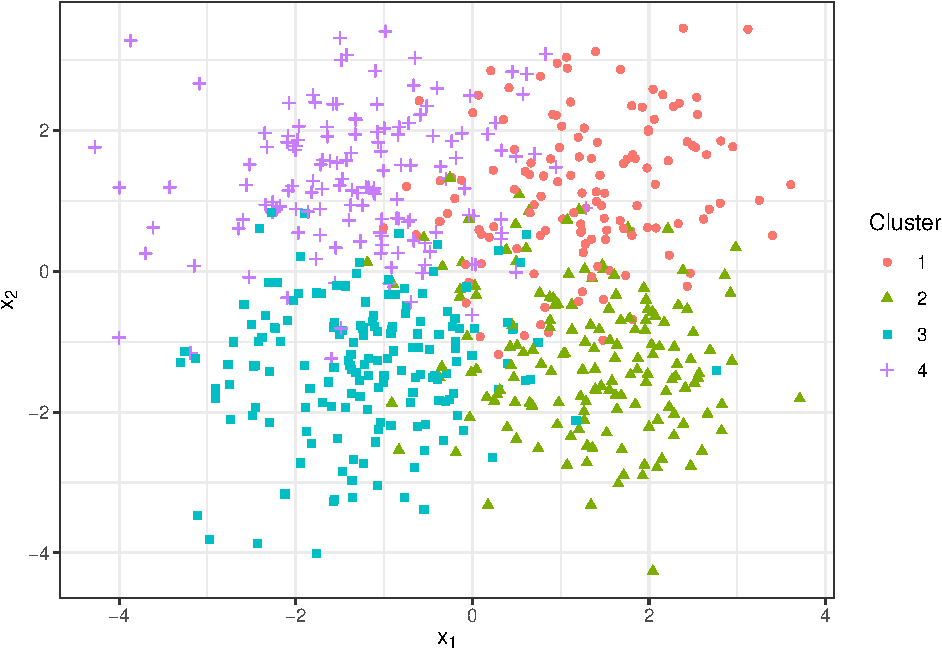
\includegraphics[width=1\linewidth]{man/figures/README-unnamed-chunk-8-1}

Let's run the MCMC:

\begin{Shaded}
\begin{Highlighting}[]
\FunctionTok{set.seed}\NormalTok{(}\DecValTok{4321}\NormalTok{)}
\DocumentationTok{\#\#\# Parameters for DP mixture}
\NormalTok{alpha }\OtherTok{=} \DecValTok{1}
\CommentTok{\# using Fraley and Raftery recommendation}
\NormalTok{a\_x}\OtherTok{=}\FunctionTok{rep}\NormalTok{((p}\SpecialCharTok{+}\DecValTok{2}\NormalTok{)}\SpecialCharTok{/}\DecValTok{2}\NormalTok{,p)}
\NormalTok{khat }\OtherTok{=} \DecValTok{4}
\NormalTok{b\_x}\OtherTok{=} \FunctionTok{rep}\NormalTok{(}\FunctionTok{mean}\NormalTok{(}\FunctionTok{apply}\NormalTok{(Y,}\DecValTok{2}\NormalTok{,var))}\SpecialCharTok{/}\NormalTok{(khat}\SpecialCharTok{\^{}}\NormalTok{(}\DecValTok{2}\SpecialCharTok{/}\NormalTok{p))}\SpecialCharTok{/}\DecValTok{2}\NormalTok{,p)}

\DocumentationTok{\#\#\# Parameters for MCMC function}
\NormalTok{S}\OtherTok{=}\DecValTok{10000}
\NormalTok{thin }\OtherTok{=} \DecValTok{1}
\NormalTok{tot }\OtherTok{=}\NormalTok{ S}\SpecialCharTok{*}\NormalTok{thin}
\NormalTok{burnin}\OtherTok{=}\DecValTok{5000}

\NormalTok{est\_model }\OtherTok{\textless{}{-}}\NormalTok{ BNPmix}\SpecialCharTok{::}\FunctionTok{PYdensity}\NormalTok{(}\AttributeTok{y =}\NormalTok{ Y,}
                       \AttributeTok{mcmc =} \FunctionTok{list}\NormalTok{(}\AttributeTok{niter =}\NormalTok{ burnin }\SpecialCharTok{+}\NormalTok{ tot,}
                                   \AttributeTok{nburn =}\NormalTok{ burnin,}
                                   \AttributeTok{model =} \StringTok{"DLS"}\NormalTok{,}
                                   \AttributeTok{hyper =} \ConstantTok{FALSE}
\NormalTok{                                   ),}
                       \AttributeTok{prior =} \FunctionTok{list}\NormalTok{(}
                         \AttributeTok{k0 =} \FloatTok{0.1}\SpecialCharTok{*}\FunctionTok{rep}\NormalTok{(}\DecValTok{1}\NormalTok{,p),}
                         \AttributeTok{a0 =}\NormalTok{ a\_x,}
                         \AttributeTok{b0 =}\NormalTok{ b\_x,}
                         \AttributeTok{strength =}\NormalTok{ alpha,}
                         \AttributeTok{discount =} \DecValTok{0}\NormalTok{),}
                       \AttributeTok{output =} \FunctionTok{list}\NormalTok{(}\AttributeTok{out\_type =} \StringTok{"FULL"}\NormalTok{, }\AttributeTok{out\_param =} \ConstantTok{TRUE}\NormalTok{))}
\CommentTok{\#\textgreater{} Completed:   1500/15000 {-} in 0.545666 sec}
\CommentTok{\#\textgreater{} Completed:   3000/15000 {-} in 1.05373 sec}
\CommentTok{\#\textgreater{} Completed:   4500/15000 {-} in 1.55122 sec}
\CommentTok{\#\textgreater{} Completed:   6000/15000 {-} in 2.20961 sec}
\CommentTok{\#\textgreater{} Completed:   7500/15000 {-} in 2.85217 sec}
\CommentTok{\#\textgreater{} Completed:   9000/15000 {-} in 3.56757 sec}
\CommentTok{\#\textgreater{} Completed:   10500/15000 {-} in 4.30253 sec}
\CommentTok{\#\textgreater{} Completed:   12000/15000 {-} in 4.9957 sec}
\CommentTok{\#\textgreater{} Completed:   13500/15000 {-} in 5.66437 sec}
\CommentTok{\#\textgreater{} Completed:   15000/15000 {-} in 6.35822 sec}
\CommentTok{\#\textgreater{} }
\CommentTok{\#\textgreater{} Estimation done in 6.35826 seconds}
\NormalTok{cls.draw }\OtherTok{=}\NormalTok{ est\_model}\SpecialCharTok{$}\NormalTok{clust}
\NormalTok{psm}\OtherTok{=}\NormalTok{mcclust}\SpecialCharTok{::}\FunctionTok{comp.psm}\NormalTok{(cls.draw}\SpecialCharTok{+}\DecValTok{1}\NormalTok{)}
\end{Highlighting}
\end{Shaded}

Let's inspect the minVI estimator:

\begin{Shaded}
\begin{Highlighting}[]
\NormalTok{z\_minVI }\OtherTok{=}\NormalTok{ salso}\SpecialCharTok{::}\FunctionTok{salso}\NormalTok{(}\AttributeTok{x =}\NormalTok{ cls.draw, }\AttributeTok{loss =} \FunctionTok{VI}\NormalTok{(}\AttributeTok{a =} \FloatTok{0.9}\NormalTok{))}
\FunctionTok{table}\NormalTok{(z\_minVI)}
\CommentTok{\#\textgreater{} z\_minVI}
\CommentTok{\#\textgreater{}   1   2 }
\CommentTok{\#\textgreater{} 501  99}

\NormalTok{df }\OtherTok{=} \FunctionTok{data.frame}\NormalTok{(}\AttributeTok{x1 =}\NormalTok{ Y[,}\DecValTok{1}\NormalTok{],}
                \AttributeTok{x2 =}\NormalTok{ Y[,}\DecValTok{2}\NormalTok{],}
                \AttributeTok{Cluster =}\NormalTok{ z\_minVI)}
\NormalTok{df}\SpecialCharTok{$}\NormalTok{Cluster }\OtherTok{=} \FunctionTok{as.factor}\NormalTok{(df}\SpecialCharTok{$}\NormalTok{Cluster)}

\FunctionTok{ggplot}\NormalTok{(df)}\SpecialCharTok{+}
  \FunctionTok{geom\_point}\NormalTok{(}\FunctionTok{aes}\NormalTok{(}\AttributeTok{x =}\NormalTok{ x1, }\AttributeTok{y =}\NormalTok{ x2, }\AttributeTok{color =}\NormalTok{ Cluster, }\AttributeTok{shape =}\NormalTok{ Cluster)) }\SpecialCharTok{+}
  \FunctionTok{ylab}\NormalTok{(}\FunctionTok{expression}\NormalTok{(}\StringTok{"x"}\NormalTok{[}\DecValTok{2}\NormalTok{]))}\SpecialCharTok{+}\FunctionTok{xlab}\NormalTok{(}\FunctionTok{expression}\NormalTok{(}\StringTok{"x"}\NormalTok{[}\DecValTok{1}\NormalTok{]))}\SpecialCharTok{+}
  \FunctionTok{theme\_bw}\NormalTok{()}
\end{Highlighting}
\end{Shaded}

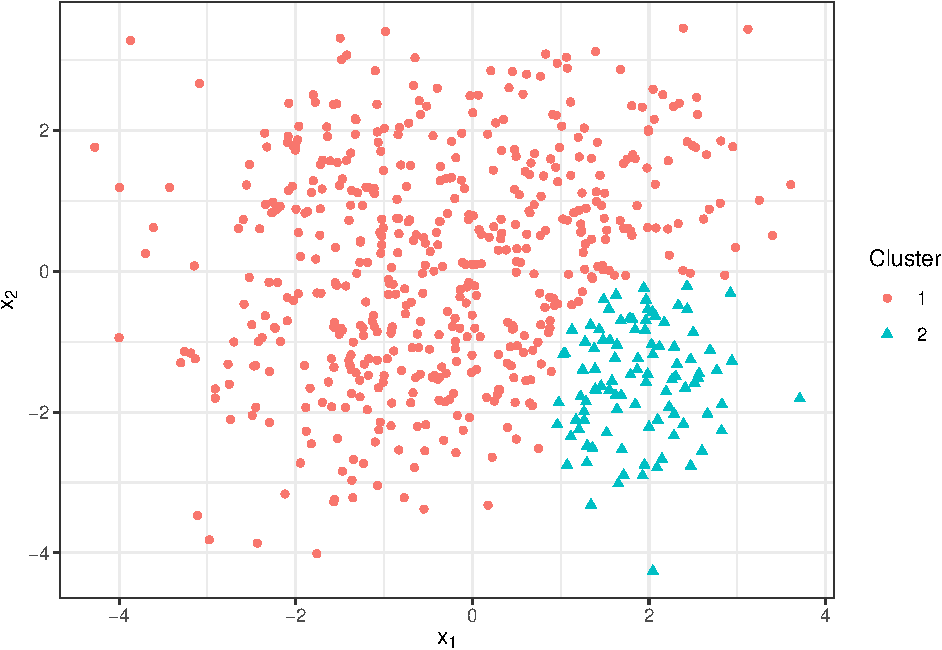
\includegraphics[width=1\linewidth]{man/figures/README-unnamed-chunk-10-1}

The minVI estimator is the partition with two cluster.

\begin{Shaded}
\begin{Highlighting}[]
\NormalTok{superheat}\SpecialCharTok{::}\FunctionTok{superheat}\NormalTok{(psm,}
                     \AttributeTok{heat.pal =} \FunctionTok{c}\NormalTok{(}\StringTok{"white"}\NormalTok{, }\StringTok{"yellow"}\NormalTok{, }\StringTok{"red"}\NormalTok{),}
                     \AttributeTok{heat.pal.values =} \FunctionTok{c}\NormalTok{(}\DecValTok{0}\NormalTok{,.}\DecValTok{5}\NormalTok{,}\DecValTok{1}\NormalTok{),}
                     \AttributeTok{pretty.order.cols =} \ConstantTok{TRUE}\NormalTok{,}
                     \AttributeTok{pretty.order.rows =} \ConstantTok{TRUE}\NormalTok{,}
                     \AttributeTok{membership.rows =}\NormalTok{ z\_minVI,}
                     \AttributeTok{membership.cols =}\NormalTok{ z\_minVI,}
                     \AttributeTok{bottom.label.text.size =} \DecValTok{4}\NormalTok{,}
                     \AttributeTok{left.label.text.size =} \DecValTok{4}\NormalTok{)}
\CommentTok{\#\textgreater{} Warning: Using \textasciigrave{}size\textasciigrave{} aesthetic for lines was deprecated in ggplot2 3.4.0.}
\CommentTok{\#\textgreater{} i Please use \textasciigrave{}linewidth\textasciigrave{} instead.}
\CommentTok{\#\textgreater{} i The deprecated feature was likely used in the superheat package.}
\CommentTok{\#\textgreater{}   Please report the issue to the authors.}
\CommentTok{\#\textgreater{} This warning is displayed once every 8 hours.}
\CommentTok{\#\textgreater{} Call \textasciigrave{}lifecycle::last\_lifecycle\_warnings()\textasciigrave{} to see where this warning was}
\CommentTok{\#\textgreater{} generated.}
\end{Highlighting}
\end{Shaded}

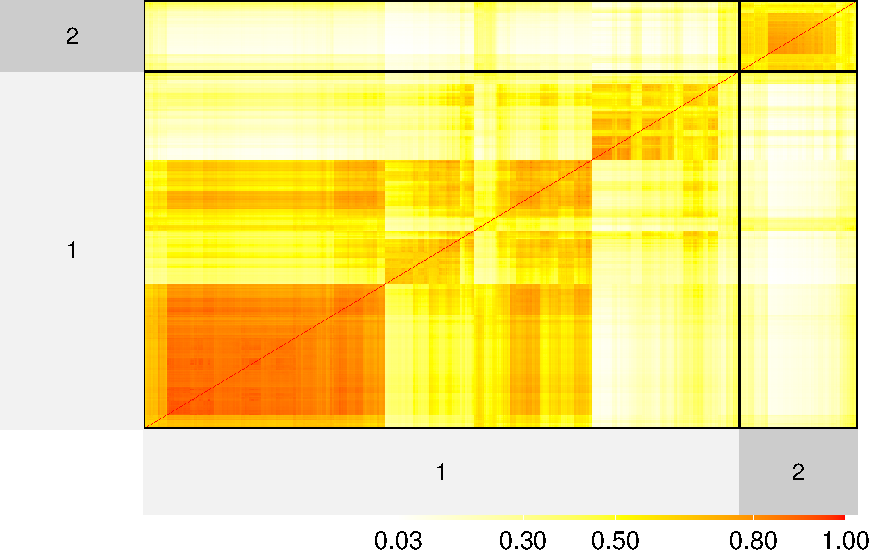
\includegraphics[width=1\linewidth]{man/figures/README-unnamed-chunk-11-1}

However the posterior similarity matrix shows a potential four-cluster
pattern, with moderate posterior uncertainty.

Let's use the \texttt{elbow} function to choose the number of particles
\(L\) that summarizes the posterior with multiple point estimates under
WASABI framework with the elbow method :

\begin{Shaded}
\begin{Highlighting}[]
\FunctionTok{set.seed}\NormalTok{(}\DecValTok{123}\NormalTok{)}
\NormalTok{out\_elbow }\OtherTok{\textless{}{-}} \FunctionTok{elbow}\NormalTok{(cls.draw, }\AttributeTok{L\_max =} \DecValTok{6}\NormalTok{, }\AttributeTok{psm =}\NormalTok{ psm,}
                   \AttributeTok{multi.start =} \DecValTok{1}\NormalTok{,}
                   \AttributeTok{method.init =} \StringTok{"topvi"}\NormalTok{, }\AttributeTok{method =} \StringTok{"salso"}\NormalTok{,}
                   \AttributeTok{loss =} \StringTok{"VI"}\NormalTok{, }\AttributeTok{a  =} \FloatTok{0.9}\NormalTok{)}
\CommentTok{\#\textgreater{} Completed  1 / 6 }
\CommentTok{\#\textgreater{} Completed  2 / 6 }
\CommentTok{\#\textgreater{} Completed  3 / 6 }
\CommentTok{\#\textgreater{} Completed  4 / 6 }
\CommentTok{\#\textgreater{} Completed  5 / 6 }
\CommentTok{\#\textgreater{} Completed  6 / 6}
\FunctionTok{plot}\NormalTok{(out\_elbow}\SpecialCharTok{$}\NormalTok{wass\_vec, }\AttributeTok{type =} \StringTok{"b"}\NormalTok{, }\AttributeTok{ylab =} \StringTok{"Wass distance"}\NormalTok{, }\AttributeTok{xlab =} \StringTok{"Number of particles"}\NormalTok{)}
\end{Highlighting}
\end{Shaded}

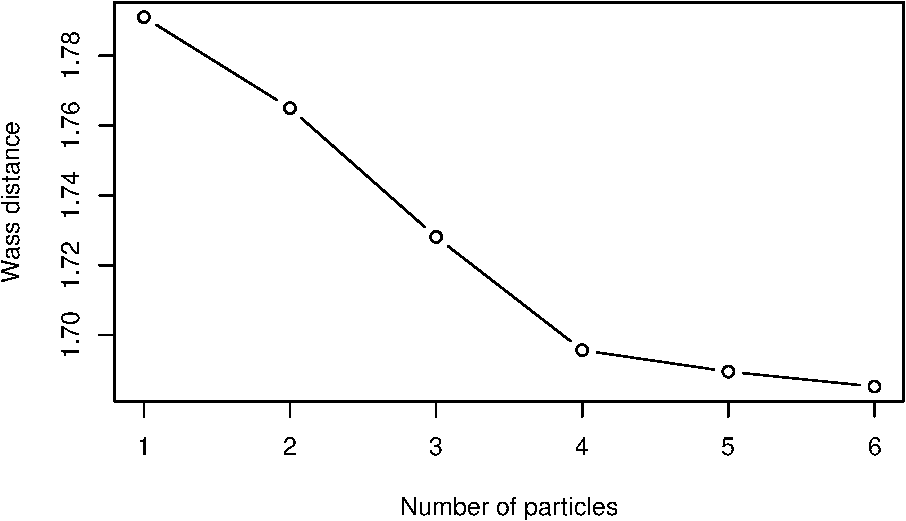
\includegraphics[width=1\linewidth]{man/figures/README-run_elbow-1}

We can then choose \(L = 4\).

\begin{Shaded}
\begin{Highlighting}[]
\NormalTok{L }\OtherTok{=} \DecValTok{4}
\NormalTok{output\_WASABI }\OtherTok{\textless{}{-}}\NormalTok{ out\_elbow}\SpecialCharTok{$}\NormalTok{output\_list[[L]]}
\end{Highlighting}
\end{Shaded}

Once the value of \(L\) is chosen, we can run another set of
initializations to see if we can find a better approximation:

\begin{Shaded}
\begin{Highlighting}[]
\NormalTok{output\_WASABI\_mb }\OtherTok{=} \FunctionTok{WASABI\_multistart}\NormalTok{(cls.draw, psm,}
                                    \AttributeTok{multi.start =} \DecValTok{25}\NormalTok{, }\AttributeTok{ncores =} \DecValTok{4}\NormalTok{,}
                                    \AttributeTok{method.init =}\StringTok{"++"}\NormalTok{, }\AttributeTok{add\_topvi =} \ConstantTok{FALSE}\NormalTok{,}
                                    \AttributeTok{method=}\StringTok{"salso"}\NormalTok{, }\AttributeTok{L=}\NormalTok{L,}
                                    \AttributeTok{mini.batch =} \DecValTok{500}\NormalTok{,}
                                    \AttributeTok{max.iter=} \DecValTok{10}\NormalTok{, }\AttributeTok{extra.iter =} \DecValTok{5}\NormalTok{,}
                                    \AttributeTok{suppress.comment=}\ConstantTok{FALSE}\NormalTok{,}
                                    \AttributeTok{swap\_countone =} \ConstantTok{TRUE}\NormalTok{,}
                                    \AttributeTok{seed =} \DecValTok{54321}\NormalTok{,}
                                    \AttributeTok{loss =} \StringTok{"VI"}\NormalTok{, }\AttributeTok{a =} \FloatTok{0.9}\NormalTok{)}
\end{Highlighting}
\end{Shaded}

We should use the solution achieving the smallest Wasserstein distance
(wass.dist):

\begin{Shaded}
\begin{Highlighting}[]
\ControlFlowTok{if}\NormalTok{(output\_WASABI\_mb}\SpecialCharTok{$}\NormalTok{wass.dist }\SpecialCharTok{\textless{}}\NormalTok{ output\_WASABI}\SpecialCharTok{$}\NormalTok{wass.dist)\{}
\NormalTok{  output\_WASABI }\OtherTok{\textless{}{-}}\NormalTok{ output\_WASABI\_mb}
\NormalTok{\}}
\FunctionTok{print}\NormalTok{(output\_WASABI}\SpecialCharTok{$}\NormalTok{wass.dist)}
\CommentTok{\#\textgreater{} [1] 1.694767}
\end{Highlighting}
\end{Shaded}

We can now visualize the particles, and there are different options:

visualize the weight for each particle

\begin{Shaded}
\begin{Highlighting}[]
\FunctionTok{ggsummary}\NormalTok{(output\_WASABI)}
\end{Highlighting}
\end{Shaded}

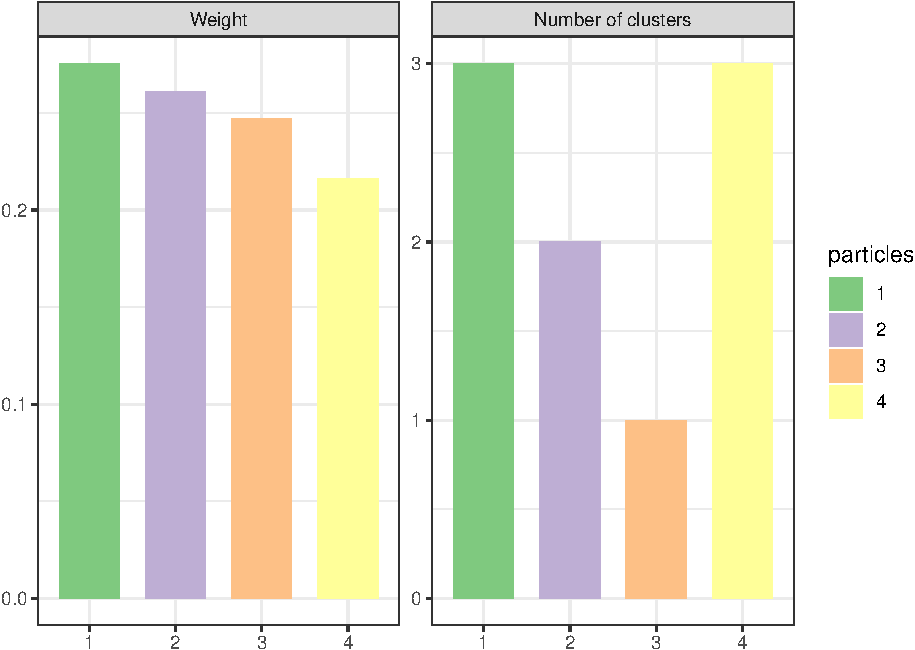
\includegraphics[width=1\linewidth]{man/figures/README-unnamed-chunk-14-1}

visualize the the range for each particle's cluster, side by side with
the histogram of the data:

\begin{Shaded}
\begin{Highlighting}[]
\FunctionTok{ggrange\_hist}\NormalTok{(output\_WASABI, Y[,}\DecValTok{2}\NormalTok{])}
\CommentTok{\#\textgreater{} \textasciigrave{}stat\_bin()\textasciigrave{} using \textasciigrave{}bins = 30\textasciigrave{}. Pick better value \textasciigrave{}binwidth\textasciigrave{}.}
\end{Highlighting}
\end{Shaded}

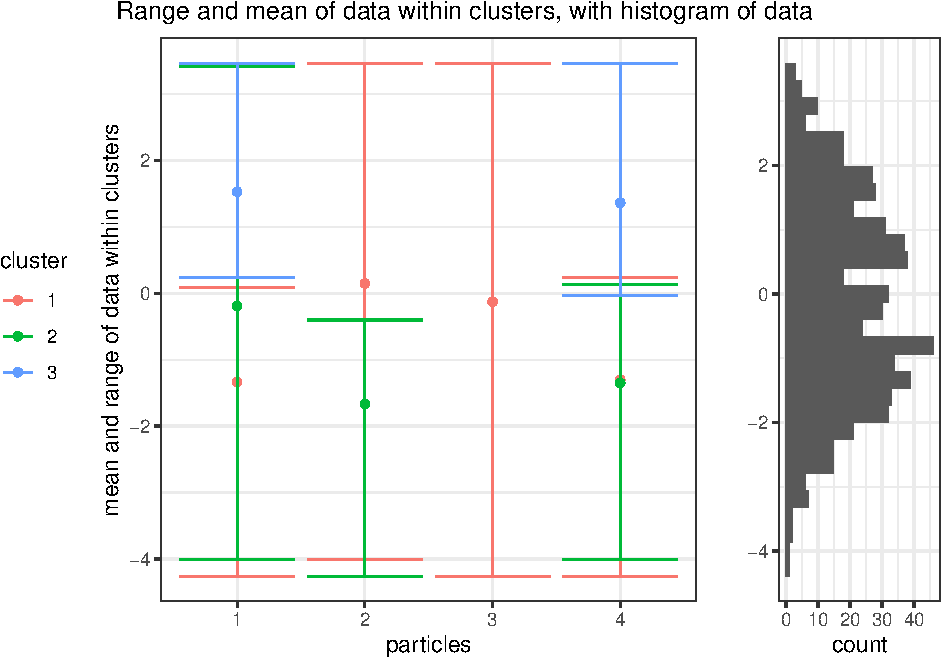
\includegraphics[width=1\linewidth]{man/figures/README-unnamed-chunk-15-1}

visualize the data with the particles' cluster assignment, as a
scatterplot (by adding some jitter in the y-axis):

\begin{Shaded}
\begin{Highlighting}[]
\FunctionTok{ggscatter\_grid2d}\NormalTok{(output\_WASABI, Y)}
\end{Highlighting}
\end{Shaded}

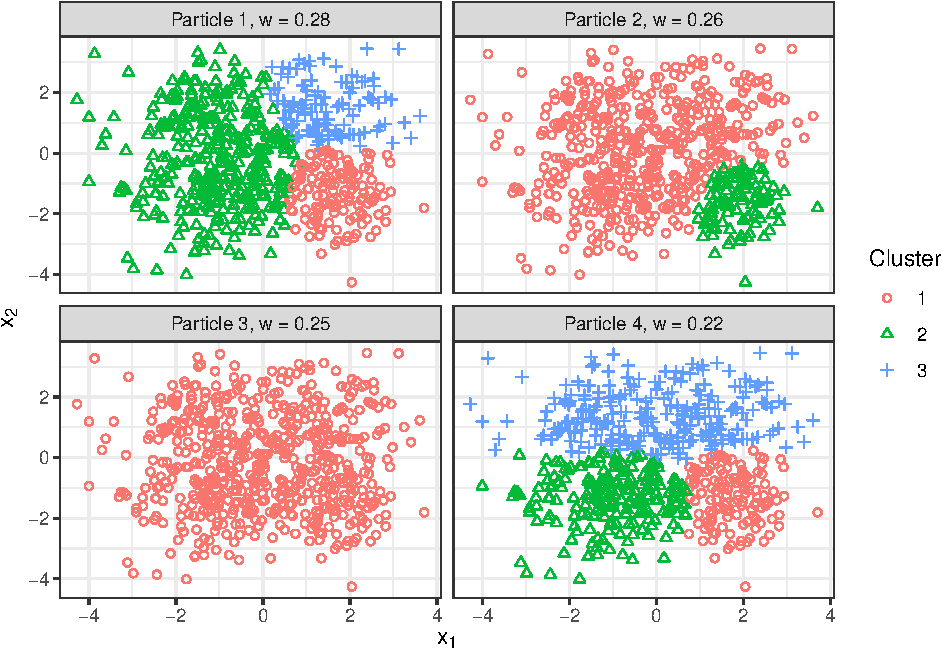
\includegraphics[width=1\linewidth]{man/figures/README-unnamed-chunk-16-1}

We can also find the meet of the particles:

\begin{Shaded}
\begin{Highlighting}[]
\NormalTok{output\_meet }\OtherTok{=} \FunctionTok{cls.meet}\NormalTok{(output\_WASABI}\SpecialCharTok{$}\NormalTok{particles)}
\NormalTok{z\_meet }\OtherTok{=}\NormalTok{ output\_meet}\SpecialCharTok{$}\NormalTok{cls.m}
\end{Highlighting}
\end{Shaded}

\begin{Shaded}
\begin{Highlighting}[]
\NormalTok{df\_tmp }\OtherTok{\textless{}{-}} \FunctionTok{data.frame}\NormalTok{(}\AttributeTok{x1 =}\NormalTok{ Y[,}\DecValTok{1}\NormalTok{],}
           \AttributeTok{x2 =}\NormalTok{ Y[,}\DecValTok{2}\NormalTok{],}
           \AttributeTok{Cluster =}\NormalTok{ z\_meet)}
\FunctionTok{ggplot}\NormalTok{(df\_tmp) }\SpecialCharTok{+}
  \FunctionTok{geom\_point}\NormalTok{(}\FunctionTok{aes}\NormalTok{(}\AttributeTok{x =}\NormalTok{ x1,}\AttributeTok{y =}\NormalTok{ x2,}
                 \AttributeTok{color =} \FunctionTok{as.factor}\NormalTok{(Cluster))) }\SpecialCharTok{+}
  \FunctionTok{theme\_bw}\NormalTok{() }\SpecialCharTok{+}
  \FunctionTok{xlab}\NormalTok{(}\FunctionTok{expression}\NormalTok{(}\StringTok{"x"}\NormalTok{[}\DecValTok{1}\NormalTok{])) }\SpecialCharTok{+} \FunctionTok{ylab}\NormalTok{(}\FunctionTok{expression}\NormalTok{(}\StringTok{"x"}\NormalTok{[}\DecValTok{2}\NormalTok{]))}\SpecialCharTok{+}
  \FunctionTok{ggtitle}\NormalTok{(}\StringTok{"Particles meet"}\NormalTok{)}\SpecialCharTok{+}\FunctionTok{theme}\NormalTok{(}\AttributeTok{legend.box =} \StringTok{"horizotal"}\NormalTok{)}
\end{Highlighting}
\end{Shaded}

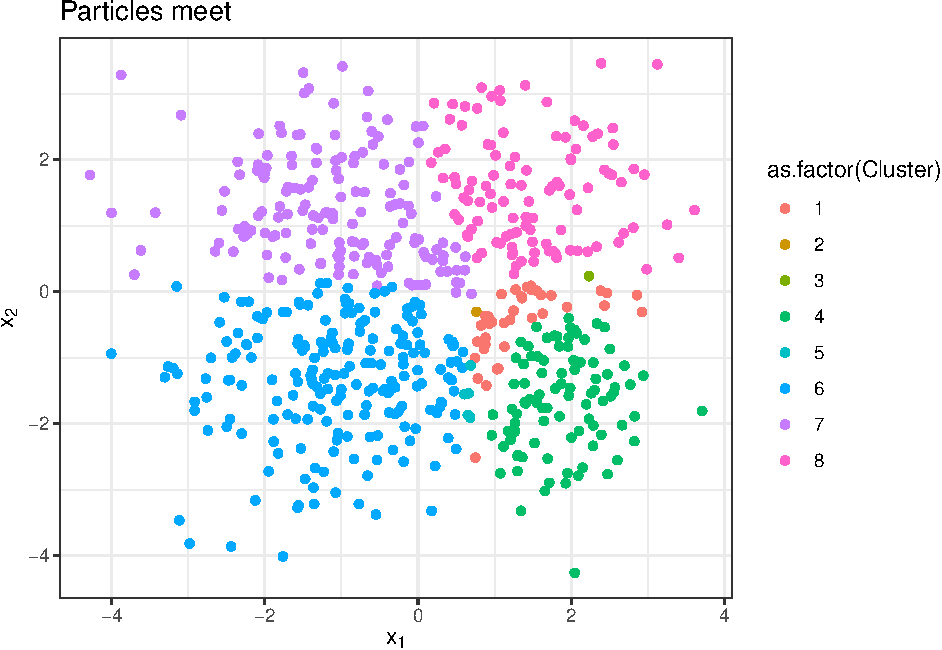
\includegraphics[width=1\linewidth]{man/figures/README-unnamed-chunk-18-1}

Let's now look at the WASABI-approximation of the posterior similarity
matrix, which is defined on the meet's clusters:

\begin{Shaded}
\begin{Highlighting}[]
\NormalTok{psm.m }\OtherTok{=} \FunctionTok{psm.meet}\NormalTok{(z\_meet, output\_WASABI)}
\NormalTok{Km }\OtherTok{\textless{}{-}} \FunctionTok{nrow}\NormalTok{(psm.m)}
\FunctionTok{colnames}\NormalTok{(psm.m) }\OtherTok{\textless{}{-}} \DecValTok{1}\SpecialCharTok{:}\NormalTok{Km; }\FunctionTok{rownames}\NormalTok{(psm.m) }\OtherTok{\textless{}{-}} \DecValTok{1}\SpecialCharTok{:}\NormalTok{Km}
\end{Highlighting}
\end{Shaded}

Let's plot it and simultaneously compare the meet with one of the
particles (e.g.~2) We will now import \texttt{dplyr} to use the pipe,
but equivalent base R code can be used:

\begin{Shaded}
\begin{Highlighting}[]
\FunctionTok{library}\NormalTok{(dplyr)}
\CommentTok{\#\textgreater{} }
\CommentTok{\#\textgreater{} Attaching package: \textquotesingle{}dplyr\textquotesingle{}}
\CommentTok{\#\textgreater{} The following objects are masked from \textquotesingle{}package:stats\textquotesingle{}:}
\CommentTok{\#\textgreater{} }
\CommentTok{\#\textgreater{}     filter, lag}
\CommentTok{\#\textgreater{} The following objects are masked from \textquotesingle{}package:base\textquotesingle{}:}
\CommentTok{\#\textgreater{} }
\CommentTok{\#\textgreater{}     intersect, setdiff, setequal, union}
\NormalTok{i }\OtherTok{=} \DecValTok{2}
\NormalTok{part\_cl }\OtherTok{=}\NormalTok{ output\_WASABI}\SpecialCharTok{$}\NormalTok{particles[i,]}
\NormalTok{tb\_meettop }\OtherTok{=} \FunctionTok{table}\NormalTok{(part\_cl,z\_meet)}
\NormalTok{lbs\_top }\OtherTok{=} \FunctionTok{rownames}\NormalTok{(tb\_meettop)[}\FunctionTok{as.factor}\NormalTok{(}\FunctionTok{apply}\NormalTok{(tb\_meettop, }\DecValTok{2}\NormalTok{, which.max))]}

\NormalTok{tmp }\OtherTok{=}\NormalTok{ reshape2}\SpecialCharTok{::}\FunctionTok{melt}\NormalTok{(}\FunctionTok{as.matrix}\NormalTok{(}\FunctionTok{as.data.frame.matrix}\NormalTok{(tb\_meettop))) }\SpecialCharTok{\%\textgreater{}\%}
  \FunctionTok{arrange}\NormalTok{(Var1,}\SpecialCharTok{{-}}\NormalTok{value) }\SpecialCharTok{\%\textgreater{}\%} \FunctionTok{filter}\NormalTok{(value }\SpecialCharTok{\textgreater{}} \DecValTok{0}\NormalTok{) }\SpecialCharTok{\%\textgreater{}\%} \FunctionTok{pull}\NormalTok{(Var2)}

\NormalTok{superheat}\SpecialCharTok{::}\FunctionTok{superheat}\NormalTok{(psm.m,}
                     \AttributeTok{title =} \FunctionTok{paste}\NormalTok{(}\StringTok{\textquotesingle{}Meet vs Particle\textquotesingle{}}\NormalTok{,i),}
                     \AttributeTok{heat.pal =} \FunctionTok{c}\NormalTok{(}\StringTok{"white"}\NormalTok{, }\StringTok{"yellow"}\NormalTok{, }\StringTok{"red"}\NormalTok{),}
                     \AttributeTok{heat.pal.values =} \FunctionTok{c}\NormalTok{(}\DecValTok{0}\NormalTok{,.}\DecValTok{5}\NormalTok{,}\DecValTok{1}\NormalTok{),}
                     \AttributeTok{heat.lim =} \FunctionTok{c}\NormalTok{(}\DecValTok{0}\NormalTok{,}\DecValTok{1}\NormalTok{), }\CommentTok{\# this is important!!}
                     \AttributeTok{row.title =} \FunctionTok{paste}\NormalTok{(}\StringTok{\textquotesingle{}Particle\textquotesingle{}}\NormalTok{,i),}
                     \AttributeTok{column.title =} \FunctionTok{paste}\NormalTok{(}\StringTok{\textquotesingle{}Meet\textquotesingle{}}\NormalTok{),}
                     \AttributeTok{membership.rows =} \FunctionTok{as.numeric}\NormalTok{(lbs\_top),}
                     \AttributeTok{order.cols =}\NormalTok{ tmp,}
                     \AttributeTok{order.rows =}\NormalTok{ tmp)}
\end{Highlighting}
\end{Shaded}

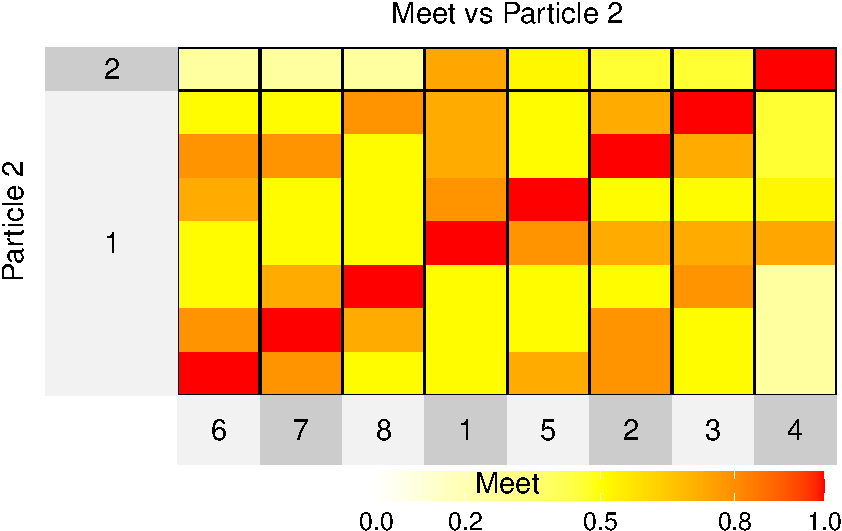
\includegraphics[width=1\linewidth]{man/figures/README-unnamed-chunk-20-1}

We can also look at the Generalized VI contribution of each point when
comparing two partitions (e.g.~particle 2 and particle 3):

\begin{Shaded}
\begin{Highlighting}[]
\NormalTok{VI\_23 }\OtherTok{=} \FunctionTok{vi.contribution}\NormalTok{(output\_WASABI}\SpecialCharTok{$}\NormalTok{particles[}\DecValTok{2}\NormalTok{,],output\_WASABI}\SpecialCharTok{$}\NormalTok{particles[}\DecValTok{3}\NormalTok{,], }\AttributeTok{a =} \FloatTok{0.9}\NormalTok{)}

\CommentTok{\# manually specify shape codes (mix of open and filled)}
\NormalTok{shape\_values }\OtherTok{\textless{}{-}} \FunctionTok{c}\NormalTok{(}\DecValTok{0}\SpecialCharTok{:}\DecValTok{9}\NormalTok{, }\DecValTok{15}\SpecialCharTok{:}\DecValTok{20}\NormalTok{)}

\FunctionTok{ggplot}\NormalTok{() }\SpecialCharTok{+}
  \FunctionTok{geom\_point}\NormalTok{(}\FunctionTok{aes}\NormalTok{(}\AttributeTok{x =}\NormalTok{ Y[,}\DecValTok{1}\NormalTok{],}
                 \AttributeTok{y =}\NormalTok{ Y[,}\DecValTok{2}\NormalTok{],}
                 \AttributeTok{color =}\NormalTok{ VI\_23,}
                 \AttributeTok{shape =} \FunctionTok{as.factor}\NormalTok{(z\_meet))) }\SpecialCharTok{+}
  \FunctionTok{scale\_shape\_manual}\NormalTok{(}\AttributeTok{values =}\NormalTok{ shape\_values) }\SpecialCharTok{+}
  \FunctionTok{theme\_bw}\NormalTok{() }\SpecialCharTok{+}
  \FunctionTok{scale\_color\_distiller}\NormalTok{(}\AttributeTok{name =} \StringTok{"GVI"}\NormalTok{,}\AttributeTok{palette =} \StringTok{"OrRd"}\NormalTok{,}\AttributeTok{direction =} \DecValTok{1}\NormalTok{)}\SpecialCharTok{+}
  \FunctionTok{guides}\NormalTok{(}\AttributeTok{shape =} \FunctionTok{guide\_legend}\NormalTok{(}\AttributeTok{title=}\StringTok{"Meet}\SpecialCharTok{\textbackslash{}n}\StringTok{cluster"}\NormalTok{)) }\SpecialCharTok{+}
  \FunctionTok{xlab}\NormalTok{(}\FunctionTok{expression}\NormalTok{(}\StringTok{"x"}\NormalTok{[}\DecValTok{1}\NormalTok{])) }\SpecialCharTok{+} \FunctionTok{ylab}\NormalTok{(}\FunctionTok{expression}\NormalTok{(}\StringTok{"x"}\NormalTok{[}\DecValTok{2}\NormalTok{])) }\SpecialCharTok{+}
  \FunctionTok{ggtitle}\NormalTok{(}\StringTok{"Generalized VI Contribution between particle 2 and 3"}\NormalTok{)}
\end{Highlighting}
\end{Shaded}

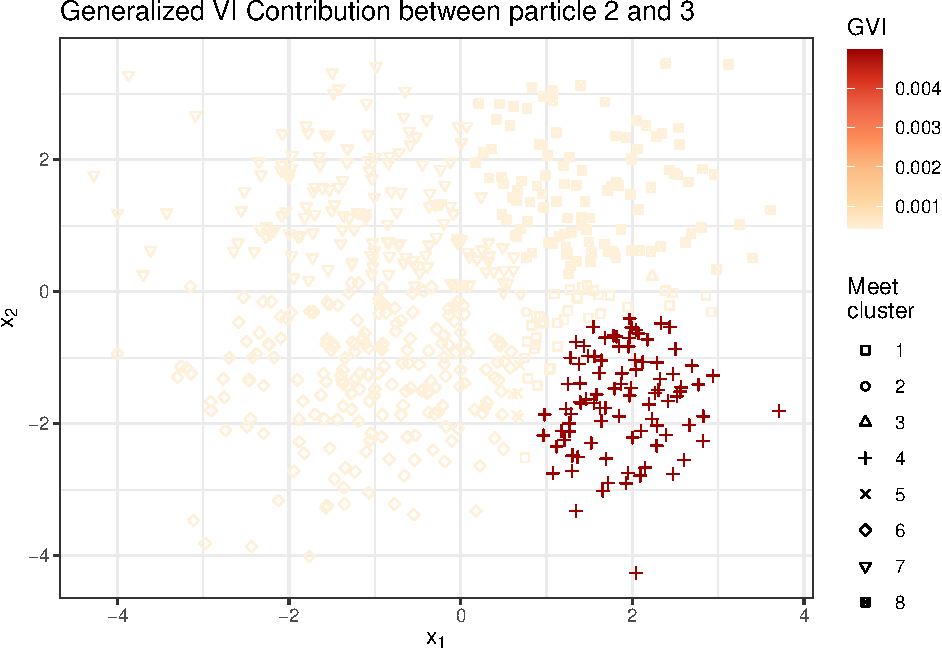
\includegraphics[width=1\linewidth]{man/figures/README-unnamed-chunk-21-1}

Or we can inspect the Expected Generalized VI Contribution (EVI) for a
given estimator, such as the meet of the particles

\begin{Shaded}
\begin{Highlighting}[]
\NormalTok{ec\_full }\OtherTok{=} \FunctionTok{evi.contribution}\NormalTok{(cls.draw, z\_meet, }\AttributeTok{a =} \FloatTok{0.9}\NormalTok{)}

\FunctionTok{data.frame}\NormalTok{(}\AttributeTok{x1 =}\NormalTok{ Y[,}\DecValTok{1}\NormalTok{],}
           \AttributeTok{x2 =}\NormalTok{ Y[,}\DecValTok{2}\NormalTok{],}
           \AttributeTok{GVI\_full =}\NormalTok{ ec\_full,}
           \AttributeTok{Cluster =} \FunctionTok{as.factor}\NormalTok{(z\_meet)) }\SpecialCharTok{\%\textgreater{}\%}
  \FunctionTok{ggplot}\NormalTok{() }\SpecialCharTok{+}
  \FunctionTok{geom\_point}\NormalTok{(}\FunctionTok{aes}\NormalTok{(}\AttributeTok{x =}\NormalTok{ x1,}\AttributeTok{y =}\NormalTok{ x2,}
                 \AttributeTok{color =}\NormalTok{ GVI\_full,}
                 \AttributeTok{shape =}\NormalTok{ Cluster)) }\SpecialCharTok{+}
  \FunctionTok{scale\_shape\_manual}\NormalTok{(}\AttributeTok{values =}\NormalTok{ shape\_values) }\SpecialCharTok{+}
  \FunctionTok{scale\_color\_distiller}\NormalTok{(}\StringTok{"EGVIC"}\NormalTok{,}\AttributeTok{palette =} \StringTok{"OrRd"}\NormalTok{,}\AttributeTok{direction =} \DecValTok{1}\NormalTok{)}\SpecialCharTok{+}
  \CommentTok{\# scale\_shape\_manual(values= c(18, 15,4, 8,19, 10,17))+}
  \FunctionTok{theme\_bw}\NormalTok{()}\SpecialCharTok{+}\FunctionTok{theme}\NormalTok{(}\AttributeTok{legend.box =} \StringTok{"horizotal"}\NormalTok{) }\SpecialCharTok{+}
  \FunctionTok{guides}\NormalTok{(}
    \AttributeTok{shape =} \FunctionTok{guide\_legend}\NormalTok{(}\AttributeTok{title.position =} \StringTok{"top"}\NormalTok{, }\AttributeTok{ncol =} \DecValTok{3}\NormalTok{)}
\NormalTok{  )}\SpecialCharTok{+}\FunctionTok{ggtitle}\NormalTok{(}\StringTok{"EGVIC for the meet"}\NormalTok{)}
\end{Highlighting}
\end{Shaded}

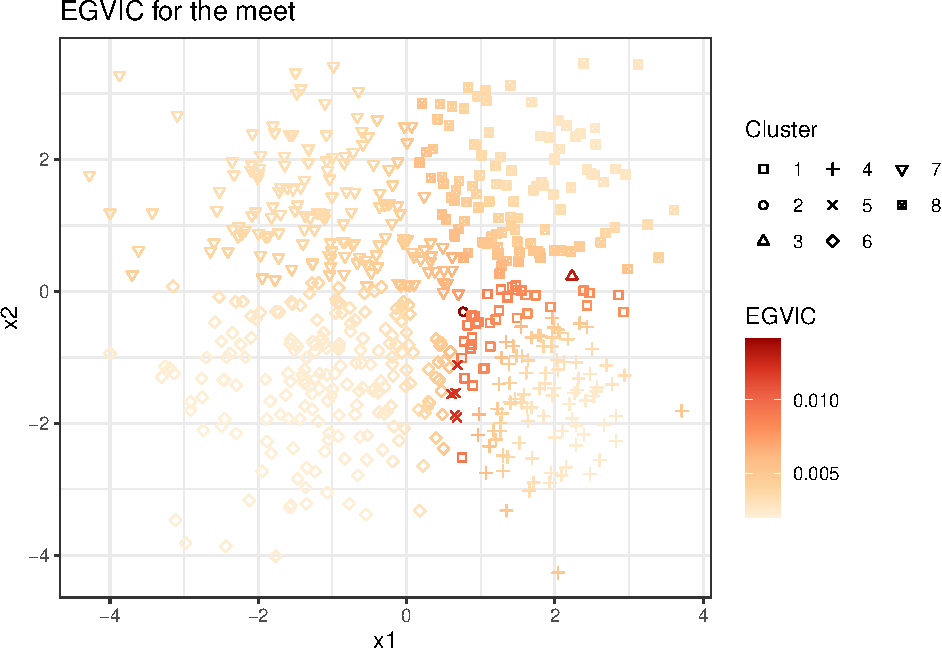
\includegraphics[width=1\linewidth]{man/figures/README-unnamed-chunk-22-1}

\end{document}
